\documentclass[17pt]{extarticle}

\usepackage[margin=1in]{geometry}
\usepackage{graphicx}
\usepackage{setspace}
\setstretch{1.1}
\usepackage{url}
\def\UrlFont{\em}
\parindent 0pt
\parskip 16pt
\pagestyle{empty}
\raggedright

\begin{document}

\begin{center}
{\large {\bf
    EEB Graduate Seminar, Fall 2016

    Theory Under Construction: \\ Building and Critiquing Biological Models
}}
\end{center}

EEB 8990, section 3 (Reg \#12123) \\
Mondays 3--4pm in Ecology 340 L or Q

\vfill
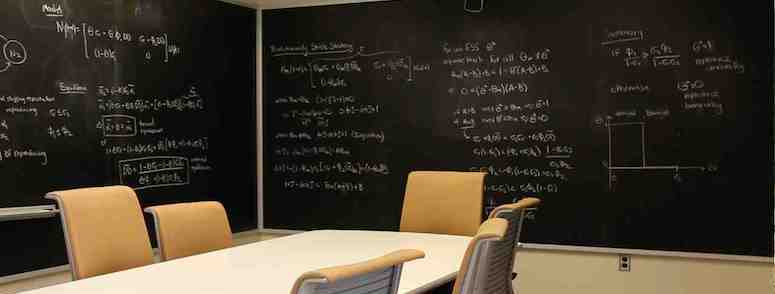
\includegraphics[width=\textwidth]{../images/chalkboards.jpg}

\vfill

Theory can help us reason through biological questions and provide rigorous connections between causal processes and observable patterns.
This class (a.k.a.\ `theory group') provides a forum for feedback on ongoing modeling work.
Each week is a discussion between the presenter(s) who describe their own work in progress, and everyone else who asks questions and offers suggestions.

\hfill \url{http://eeg.github.io/theory_lab}

\vfill

\end{document}
